\qquad O Bubble Sort (ou "ordenação por bolha") é um algoritmo de ordenação
por comparação que percorre repetidamente o vetor, comparando pares de
elementos \textit{adjacentes} e trocando-os de posição sempre que
estiverem fora de ordem. A cada passada completa pelo vetor, o maior
elemento ainda não posicionado "borbulha" até a sua posição final, de
forma análoga a uma bolha de ar subindo até a superfície — daí o nome
do algoritmo.

\qquad O algoritmo realiza, no máximo, tamanho-1 passadas. Em cada passada
\textit{i}, percorre-se o vetor comparando os pares (vetor[j],
vetor[j+1]), trocando-os quando vetor[j] > vetor[j+1]. A versão
implementada neste trabalho inclui uma otimização amplamente utilizada
na prática: uma variável de controle (\textit{trocou}) que registra se
alguma troca ocorreu durante a passada. Caso nenhuma troca tenha
ocorrido, o vetor já está ordenado e o algoritmo é interrompido
imediatamente, sem realizar as passadas restantes — isso é o que
torna o comportamento do algoritmo linear quando a entrada já está
ordenada.

\qquad A seguir apresenta-se a implementação utilizada neste trabalho, em
C++, correspondente à função \texttt{BubbleSort\_versao1}:

\begin{verbatim}
void BubbleSort_versao1(int *vetor, int tamanho) {
    int aux;
    bool trocou;
    for (int i = 0; i < tamanho - 1; i++) {
        trocou = false;
        for (int j = 0; j < tamanho - 1 - i; j++) {
            if (vetor[j] > vetor[j + 1]) {
                aux = vetor[j];
                vetor[j] = vetor[j + 1];
                vetor[j + 1] = aux;
                trocou = true;
            }
        }
        if (!trocou) break;
    }
}
\end{verbatim}

\qquad Assim como o Insertion Sort, o Bubble Sort se beneficia de entradas
já ordenadas ou quase ordenadas, apresentando desempenho linear nesse
cenário graças à parada antecipada. Por outro lado, em entradas
decrescentes ou aleatórias, o algoritmo realiza um número de
comparações da mesma ordem de grandeza do Insertion Sort, porém com um
custo maior por troca (três atribuições contra uma no deslocamento do
Insertion Sort), o que costuma torná-lo mais lento na prática, como
discutido na análise de complexidade e evidenciado nos resultados
experimentais deste capítulo.

\subsection{Teste de Mesa Manual}

\qquad Nesta seção deve ser inserida a digitalização do teste de mesa
manual do Bubble Sort, realizado à mão com um exemplo de entrada
diferente dos exemplos trabalhados em sala de aula, conforme exigido
pelo enunciado do trabalho. Substitua a imagem de exemplo abaixo pela
digitalização (foto ou escaneamento) do teste de mesa manuscrito.

\begin{figure}[htbp]
    \centering
    % Substitua o arquivo abaixo pela digitalizacao do teste de mesa manuscrito
    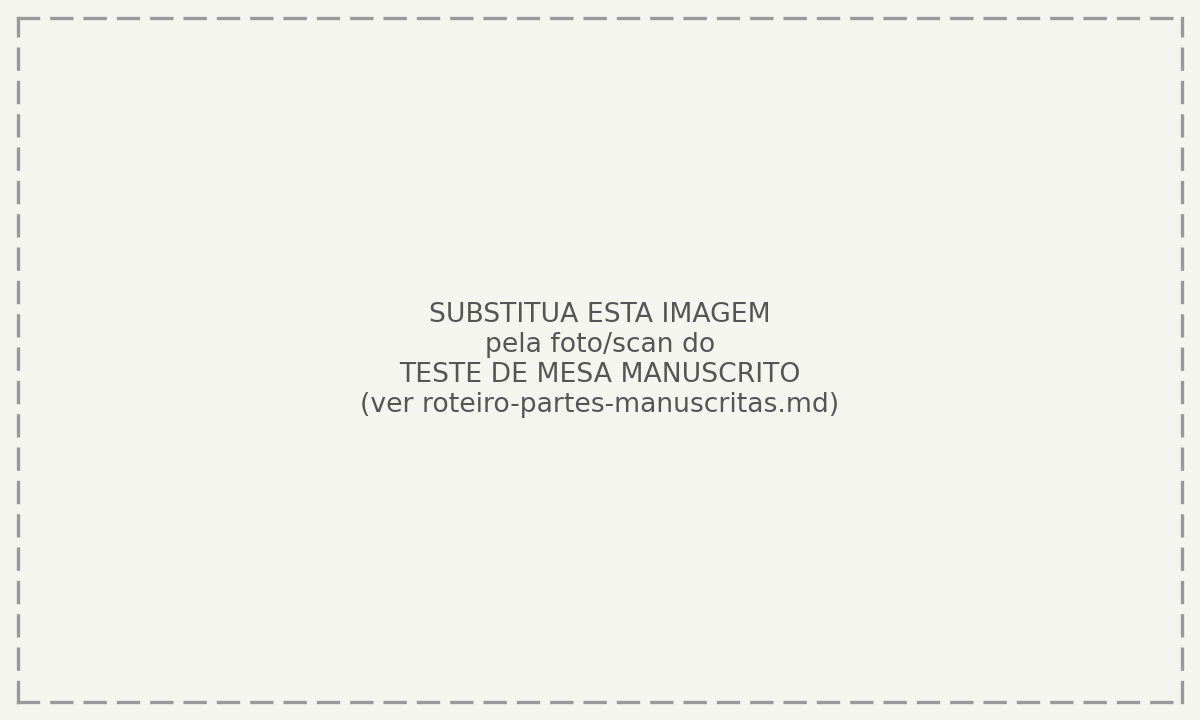
\includegraphics[width=14cm]{Imagens/Bubble Sort/teste_de_mesa.png}
    \caption{Teste de mesa manual do algoritmo Bubble Sort}
    \label{fig:teste_mesa_bubble}
\end{figure}
